
%%%%%%%%%%%%%%%%%%%%%%%%%%%%%%%%%%%%%%%%%
% Beamer Presentation
% LaTeX Template
% Version 1.0 (10/11/12)
%
% This template has been downloaded from:
% http://www.LaTeXTemplates.com
%
% License:
% CC BY-NC-SA 3.0 (http://creativecommons.org/licenses/by-nc-sa/3.0/)
%
%%%%%%%%%%%%%%%%%%%%%%%%%%%%%%%%%%%%%%%%%

%----------------------------------------------------------------------------------------
%	PACKAGES AND THEMES
%----------------------------------------------------------------------------------------

\documentclass{beamer}
\usepackage[utf8]{inputenc}
\usetheme{Copenhagen}
\usecolortheme{orchid}

\usepackage{graphicx} % Allows including images
\usepackage{booktabs} % Allows the use of \toprule, \midrule and \bottomrule in tables
%----------------------------------------------------------------------------------------
%	TITLE PAGE
%----------------------------------------------------------------------------------------

\title[TTD markers]{Time-to-death patterns in markers of age and dependency}
 
\author[Riffe et. al.]
{
T. Riffe \inst{1} \and P. H. Chung \inst{1} \and J. Spijker \inst{2} \and J.
MacInnes \inst{3} }

\institute[VFU] % (optional)
{
  \inst{1}%
  Department of Demography\\
  University of California, Berkeley
  \and
  \inst{2}%
  Wittgenstein Centre (IIASA, VID/\"OAW, WU), Vienna Institute of
  Demography/Austrian Academy of Sciences
  \and
  \inst{3}
  School of Social and Political Science\\
  University of Edinburgh
}
 
\date[Dec 2014] % (optional)
{New Measures of Age and Ageing, Dec 2014}

\begin{document}

\begin{frame}
\titlepage % Print the title page as the first slide
\end{frame}

\section{Background} % A subsection can be created just before a set of slides
% with a common theme to further break down your presentation into chunks

\begin{frame}
\frametitle{Formal to empirical}
This work was inspired by some formal results that begged the question
\begin{block}{The question}
What kinds of demographic phenomena vary in informative and empirically regular
ways by remaining years of life?
\end{block}
\end{frame}

%------------------------------------------------

\begin{frame}
\frametitle{Formal to empirical}
\begin{block}{Assumption}
Many late-life conditions are probably best described as
functions of remaining years of life.
\end{block}
\vspace{1em}
* maybe because they presage or cause death?
\end{frame}

%------------------------------------------------

\begin{frame}
\frametitle{Formal to empirical}
\begin{block}{Functions}
\textit{Function} in the sense of modellable temporal structure, not causation.
\end{block}
\end{frame}

%------------------------------------------------

\begin{frame}

\end{frame}

%------------------------------------------------

\begin{frame}
\frametitle{Multiple Columns}
\begin{columns}[c] % The "c" option specifies centered vertical alignment while the "t" option is used for top vertical alignment

\column{.45\textwidth} % Left column and width

\column{.5\textwidth} 
\end{columns}
\end{frame}

%------------------------------------------------
\section{Second Section}
%------------------------------------------------

%------------------------------------------------

\begin{frame}
\frametitle{Figure}

\begin{figure}
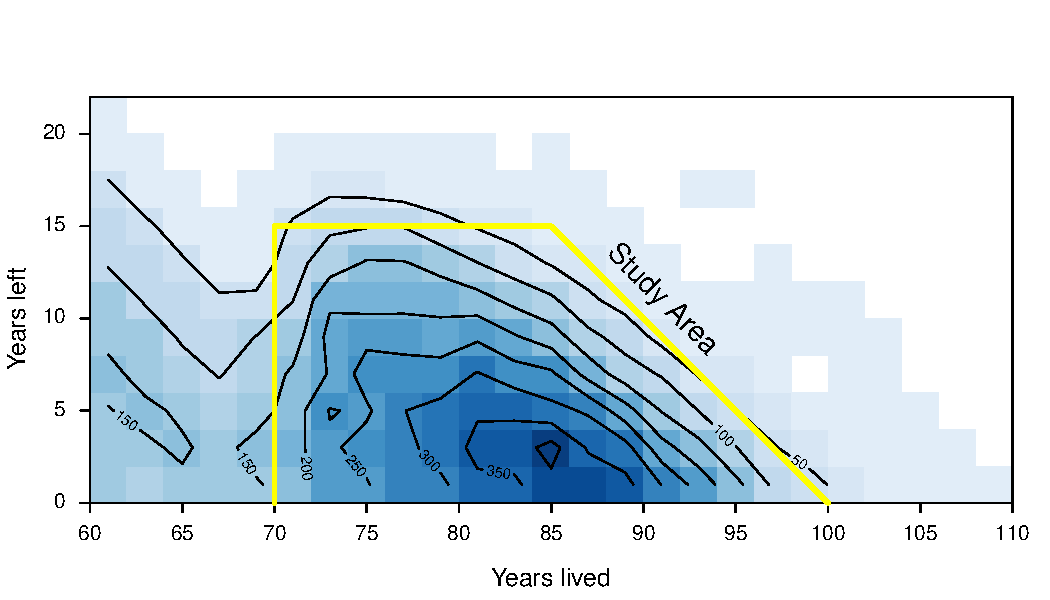
\includegraphics[width=0.8\linewidth]{Figures/CaseCountFemales}
\end{figure}
\end{frame}

%------------------------------------------------


%------------------------------------------------


%------------------------------------------------


%----------------------------------------------------------------------------------------

\end{document}





